% CEEHRC 2026 poster -- comprehensive draft, to be cut down.
%
% The conference limit is 44 in x 44 in. This draft keeps the 44 in width and runs
% taller on purpose: it carries every candidate section, and sections are removed
% from it one at a time. After a cut, set \PosterHeight to the "content ends at"
% line that the build prints, plus the 1 in bottom margin.
%
% Build: bash build.sh   (draws the panels, then runs latexmk)
\documentclass{article}
\newcommand{\PosterHeight}{84in}
\usepackage[paperwidth=44in, paperheight=\PosterHeight,
            left=1in, right=1in, top=6.4in, bottom=1in]{geometry}
\usepackage[T1]{fontenc}
\usepackage{lmodern}                 % scalable math at poster sizes
\usepackage[default]{opensans}
\usepackage{amsmath,xcolor,graphicx,tikz,qrcode,enumitem}
\usepackage[most]{tcolorbox}
\usetikzlibrary{calc}
\pagestyle{empty}
\raggedbottom
\setlength{\parindent}{0pt}
\setlength{\parskip}{0pt}

\definecolor{sfured}{HTML}{A6192E}
\definecolor{ink}{HTML}{1B2A32}
\definecolor{muted}{HTML}{5E6E78}
\definecolor{teal}{HTML}{12868C}
\definecolor{panel}{HTML}{F3F5F6}
\definecolor{rule}{HTML}{D5DBDF}

% ---- type scale, in points as printed ---------------------------------------
\newcommand{\bodysize}{\fontsize{36}{47}\selectfont}
\newcommand{\capsize}{\fontsize{31}{41}\selectfont}
\newcommand{\smallsize}{\fontsize{25}{33}\selectfont}
\newcommand{\headsize}{\fontsize{60}{72}\selectfont}

\newcommand{\sectionbar}[1]{%
  {\headsize\bfseries\color{sfured}#1}\par\vspace{0.1in}%
  {\color{sfured}\rule{\linewidth}{6pt}}\par\vspace{0.4in}}

% One panel: its graphic, then its one- or two-sentence caption.
\newcommand{\panel}[3]{% #1 width  #2 graphic  #3 caption
  \begin{minipage}[t]{#1}
    \vspace{0pt}
    \includegraphics[width=\linewidth]{#2}\par\vspace{0.25in}
    {\capsize\color{ink}#3\par}
  \end{minipage}}

\tcbset{textbox/.style={enhanced, colback=panel, colframe=panel, arc=0.25in,
  boxrule=0pt, left=0.45in, right=0.45in, top=0.35in, bottom=0.4in,
  fontupper=\bodysize\color{ink}, before skip=0pt, after skip=0pt}}
\newcommand{\boxtitle}[1]{{\fontsize{44}{54}\selectfont\bfseries\color{sfured}#1}\par\vspace{0.18in}}
\setlist[itemize]{leftmargin=1.0em, itemsep=0.15in, topsep=0.05in,
                  label={\color{sfured}\textbullet}}
\newcommand{\gap}{\hspace{1in}}

\begin{document}
% ============================================================ header ==========
% After the SFU example header: a red block from the left edge with SFU set in its
% lower right corner, then the title and the author line beside it.
\begin{tikzpicture}[remember picture, overlay]
  \coordinate (nw) at (current page.north west);
  \fill[sfured] ($(nw)+(0,-1.0in)$) rectangle ($(nw)+(9.4in,-5.0in)$);
  \node[anchor=south east, inner sep=0pt, text=white]
    at ($(nw)+(9.05in,-4.85in)$) {\fontsize{190}{190}\selectfont SFU};
  \node[anchor=south west, inner sep=0pt, text=ink]
    at ($(nw)+(10.1in,-2.75in)$)
    {\resizebox{32.9in}{!}{\bfseries Self-supervised confidence-aware denoising imputation of genomic data}};
  \node[anchor=south west, inner sep=0pt, text=ink]
    at ($(nw)+(10.1in,-4.85in)$)
    {\fontsize{80}{90}\selectfont Mehdi Foroozandeh, Abdul Rahman Diab, and Maxwell Libbrecht};
\end{tikzpicture}%
% ======================================================= problem + model ======
% Three boxes across, then the landing-page strip at full width: its labels are
% drawn at 6-8 pt, so every inch of width it gets is legibility.
\begin{minipage}[t]{13.33in}
\vspace{0pt}
\begin{tcolorbox}[textbox, equal height group=intro]
\boxtitle{The problem}
Most (cell type, assay) experiments were never run, and those that were differ in
depth, read length, run type and platform. In the ENCODE Imputation Challenge, a
baseline that averages each assay over other cell types beat all but two submitted
methods~[1].
\end{tcolorbox}
\end{minipage}\hfill
\begin{minipage}[t]{13.33in}
\vspace{0pt}
\begin{tcolorbox}[textbox, equal height group=intro]
\boxtitle{CANDI}
\textbf{C}onfidence-\textbf{A}ware \textbf{N}eural \textbf{D}enoising
\textbf{I}mputer~[2] is a self-supervised transformer over raw read counts, DNA
sequence and four experimental covariates. It predicts a distribution for every
assay in every 25\,bp bin, so each imputed value has an interval. It has no
cell-type embedding, so it runs on cell types it has never seen.
\end{tcolorbox}
\end{minipage}\hfill
\begin{minipage}[t]{13.33in}
\vspace{0pt}
\begin{tcolorbox}[textbox, equal height group=intro]
\boxtitle{Take-home}
\begin{itemize}
  \item CANDI is \textbf{1st of 26} on the ENCODE Imputation Challenge blind test.
  \item The lead needs a \textbf{24-number output correction}, fitted on training
        data only. Without it, CANDI is 14th.
  \item CANDI's intervals are calibrated, and its latent features give more
        reproducible chromatin states.
\end{itemize}
\end{tcolorbox}
\end{minipage}

\vspace{1.3in}
\sectionbar{CANDI schematic workflow}
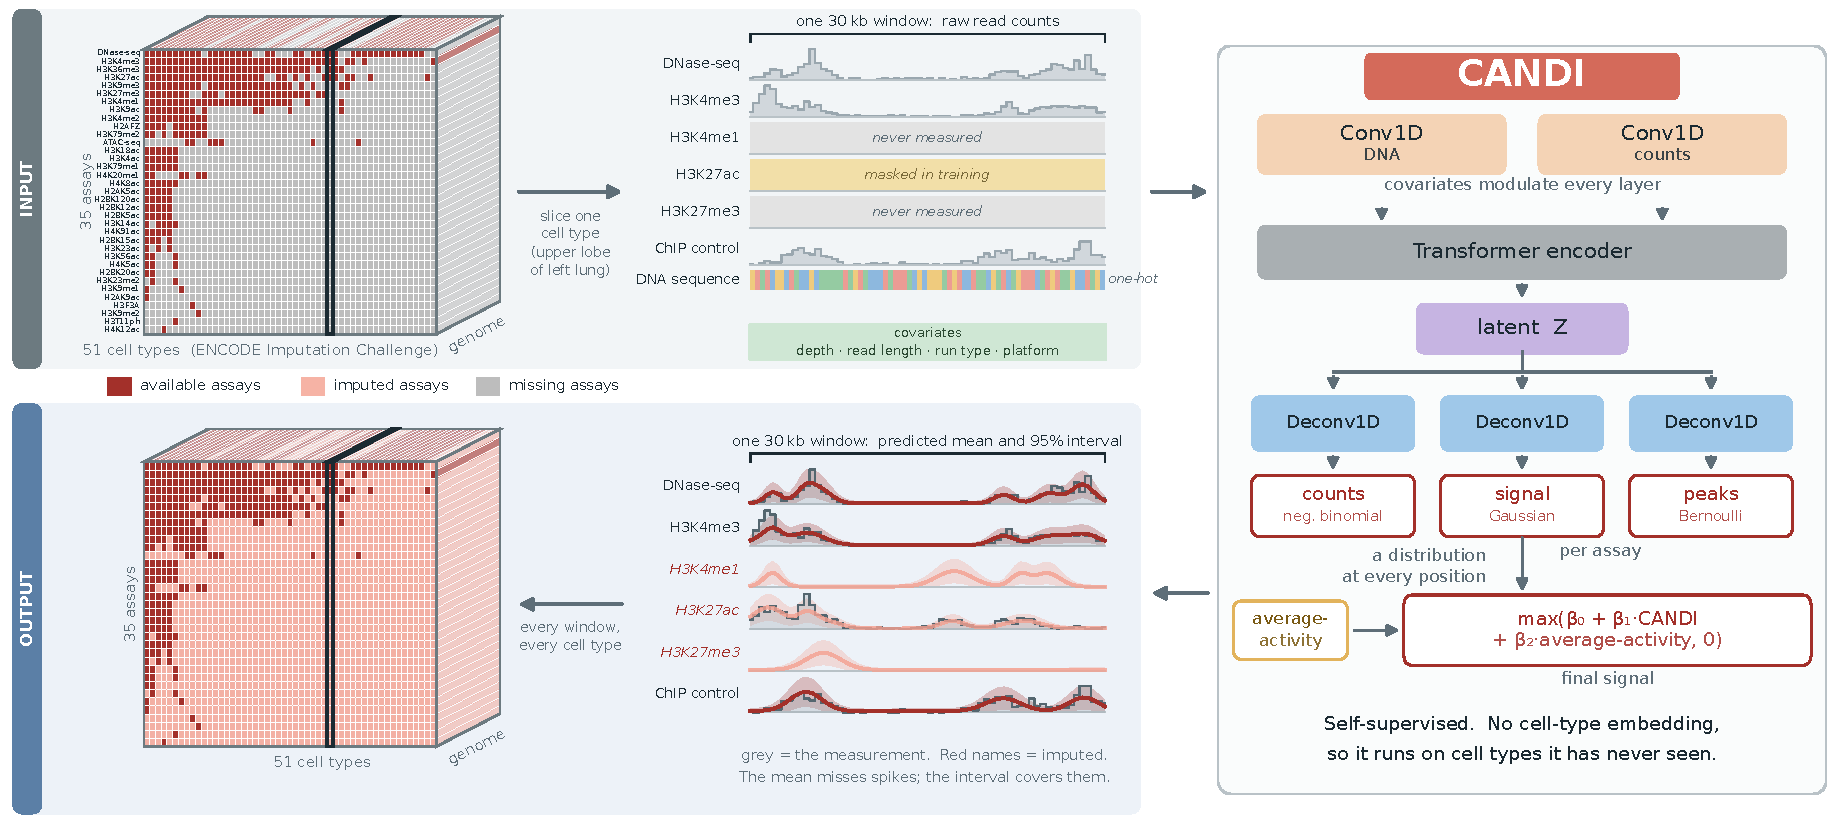
\includegraphics[width=\linewidth]{panels/ga_strip.pdf}\par\vspace{0.3in}
{\capsize\color{ink}
\textbf{Top:} one cell type is sliced out of the cell type $\times$ assay $\times$
genome tensor, and a 30\,kb window of it goes into CANDI as raw counts, DNA and
covariates. Grey assays were never measured; yellow ones are masked in training.
\textbf{Bottom:} CANDI returns a mean and a 95\% interval for every assay, and
window by window this fills every missing thread of the tensor.\par}

\vspace{1.3in}
% ================================================= published results =========
\sectionbar{Downstream utility of CANDI}
\panel{11.4in}{panels/ga_A.pdf}{\textbf{A}\enspace For DNase-seq (cell line DND-41),
the observed coverage of CANDI's intervals follows their stated confidence over the
full range.}\gap
\panel{11.7in}{panels/ga_B.pdf}{\textbf{B}\enspace Gene expression predicted from
each feature set as assays are removed. Latent features hold $r \approx 0.79$ from 13
assays down to 4; observed data falls to 0.60.}\gap
\panel{16.9in}{panels/ga_C.pdf}{\textbf{C}\enspace Agreement of SAGA chromatin-state
annotations between replicates. Latent features give the most reproducible
annotation in four of six biosamples.}

\vspace{0.35in}
{\centering
\includegraphics[width=17in]{panels/ga_legend.pdf}\par}

\vspace{1.3in}
% ================================================ the challenge ===============
\sectionbar{Fixing the signal-level shift in the ENCODE Imputation Challenge blind test}
{\bodysize\color{ink}
51 blind-test experiments (12 cell types, 8 assays), scored with the challenge's own
nine measures and ranking statistic; our scorer reproduces every published entry to a
median relative difference of $9\times10^{-10}$. CANDI's output as it comes ranks 14th,
so for each assay we pass it through one fixed layer,
$\max(\beta_0 + \beta_1\cdot\text{CANDI} + \beta_2\cdot\text{baseline},\,0)$, whose 24
numbers are fitted by least squares on the 133 training experiments only; with it,
CANDI ranks 1st.\par}
\vspace{0.8in}

\panel{13.5in}{panels/eic_leaderboard.pdf}{\textbf{D}\enspace The challenge's
leaderboard with CANDI added. CANDI is first at 0.179 (bootstrap range
0.177--0.184); the next entry scores 0.306. Bars span the ten bootstrap groups.}\gap
\panel{27.5in}{panels/eic_measures.pdf}{\textbf{E}\enspace Each of the nine measures
relative to the baseline, median over the 51 experiments. CANDI is first on
genome-wide MSE, Pearson and Spearman, and in the top 8 on five more.}

\vspace{1.3in}
% ========================================================== footer ============
{\color{rule}\rule{\linewidth}{3pt}}\par\vspace{0.5in}
\begin{minipage}[c]{34in}
{\smallsize\color{muted}
[1]~Schreiber J, Boix C, \textit{et al.} The ENCODE Imputation Challenge: a critical
assessment of methods for cross-cell type imputation of epigenomic profiles.
\textit{Genome Biol} 24:79 (2023).\par\vspace{0.12in}
[2]~Foroozandeh M, Diab AR, Libbrecht M. CANDI: self-supervised, confidence-aware
denoising imputation of genomic data. \textit{bioRxiv} 2025.01.23.634626 (2025).\par
\vspace{0.12in}
Panels D--E: blind-test scoring from the Libbrecht lab's EIC reproduction
(experiments 017, 025). \emph{Baseline} is the challenge's average-activity track.
The output correction was chosen after the challenge results were public; none of
its numbers is fitted on blind-test data.\par}
\end{minipage}\hfill
\begin{minipage}[c]{7in}
\raggedleft
{\smallsize\color{muted}mehdiforoozandeh.github.io/CANDI\par}\vspace{0.2in}
\qrcode[height=4.2in]{https://mehdiforoozandeh.github.io/CANDI/}
\end{minipage}\par
\typeout{POSTER: content ends at \the\dimexpr\pagetotal+6.4in\relax\space from the top}
\end{document}
